\subsection{Problem Description} 
    The purpose of this project is to model and solve the \textit{VLSI} problem: given a fixed-width plate and a list of 
    rectangular circuits, place them on the plate so that the length of the final device is minimized. 
    
    We faced first the easier case in which the circuits cannot be rotated and the other case on a distinct model.

    The solution of the problem gives the position of each circuit (the coordinates of the bottom left corner) and,
    in case .
    \colorbox{BurntOrange}{TODO improve ...}

% % % % % % % % % % % % % % % % % % % % % % % % % % % % % % % % % % % % % % % % % % % % % % % % % %

\subsection{Format of the Instances}
    \paragraph*{Instance Format}
        An instance of \textit{VLSI} is a text file consisting of lines of integer values. The first line gives \textit{width}, 
        which is the width of the silicon plate. The following line gives \textit{nc}, which is the number of necessary circuits 
        to place inside the plate. Then \textit{nc} lines follow, each with $w_i$ and $h_i$, representing the horizontal and 
        vertical dimensions of the \textit{i-th} circuit.

    \paragraph*{Solution Format}
        A solution of \textit{VLSI} is a text file built starting from the input file. To the first line is added the \textit{makespan},
        which is the length of the final device. The second line is kept the same while to the following \textit{nc} lines are added
        $x_i$ and $y_i$, which are the coordinates of the bottom left corner of the \textit{i-th} circuit. In case a solution is obtained 
        through the rotation of a circuit $c$, then, in the output file, the horizontal and vertical dimensions ($w_c$ and $h_c$) 
        will be swapped w.r.t. the input text file.

    \colorbox{BurntOrange}{TODO improve ...}

% % % % % % % % % % % % % % % % % % % % % % % % % % % % % % % % % % % % % % % % % % % % % % % % % %

\subsection{Shared Variables Declaration}
    In this section we list the constants and the variables that are shared in the mathematical formalization of 
    models and constraints from now on.

    Constant values:
    \begin{align*}
        nc\             &\ =\ \text{total number of circuits}                   \\
        width\          &\ =\ \text{width of the plate}                         \\
        c_i\            &\ =\ \text{index of circuit  } i                       \\
        w_i\            &\ =\ \text{width of circuit  } i                       \\
        h_i\            &\ =\ \text{height of circuit  } i                      \\
        min\_makesapan  &\ =\ \text{lower bound of \textit{makespan} variable}  \\
        max\_makesapan  &\ =\ \text{upper bound of \textit{makespan} variable}  \\
        C\              &\ =\ \bigcup_{i=1}^{nc} c_i                            \\
        CC\             &\ =\ \{(i, j) \in C \times C\ |\ i<j \}
    \end{align*}

    Variables:
    \begin{align*}
        x_i\        &\ =\ \text{x coordinate of the bottom-left corner of circuit  } i        \\
        y_i\        &\ =\ \text{y coordinate of the bottom-left corner of circuit  } i        \\
        r_i\        &\ =\ \text{boolean variable indicating if circuit \textit{i} is rotated} \\
        X\          &\ =\ \bigcup_{c=1}^{nc} x_c                                              \\
        Y\          &\ =\ \bigcup_{c=1}^{nc} y_c                                              \\
        Xcross(x)\  &\ =\ \{ c \in C\ |\ (x_c \leq x) \land (x_c + w_c > x) \}               \\
        Ycross(y)\  &\ =\ \{ c \in C\ |\ (y_c \leq y) \land (y_c + h_c > y) \}               \\
        makespan\   &\ =\ \max_{c \in C}\ y_c + h_c
    \end{align*}

    \subsubsection{Rotation}
        \colorbox{BurntOrange}{TODO missing ... se dobbiamo metterci solo $r_i$ forse questa sezione non serve ...}



\subsection{Shared Constraints Declaration}
    The following formalization will be the one followed for the CP solution and then adapted for SAT and SMT. 
    The LP model will be described later.

    \begin{align*}
           w_c > 0\ \ \land\ &\ w_c \leq width\    &\ \hspace{0.2cm} \forall c \in C \\
           h_c > 0\ \ \land\ &\ h_c \leq makespan\ &\ \hspace{0.2cm} \forall c \in C \\
        x_c \geq 0\ \ \land\ &\ x_c < width\    &\ \hspace{0.2cm} \forall c \in C \\
        y_c \geq 0\ \ \land\ &\ y_c < makespan\ &\ \hspace{0.2cm} \forall c \in C
    \end{align*}

    \begin{align}
        (x_i + w_i \leq x_j) \lor (y_i + h_i \leq y_j) &\ \ &\ \nonumber \\
        \lor\ (x_j + w_j \leq x_i) \lor (y_j + h_j \leq y_i)\ &\                \hspace{0.2cm} \forall (i,j) \in CC &\ \text{;diffn} \\
        \sum_{c \in C_x} y_c \leq makespan\ &\ \hspace{0.2cm} \forall x \in X, \forall c \in Xcross(x)\ &\ \text{;x axis} \\
        \sum_{c \in C_y} x_c \leq width\ &\ \hspace{0.2cm} \forall y \in Y, \forall c \in Ycross(y)\ &\ \text{;y axis}
    \end{align}

    \subsubsection{Symmetries}
    \colorbox{BurntOrange}{TODO controllare assolutamente formulazione delle frasi ...}


        Given a solution there are two main ways to get a different one with the same \textit{makespan}:
        swap circuits with same dimensions [Fig.\ref{fig:symmetry_swap}] or get the solution specular w.r.t. the horizontal 
        or vertical axis [Fig.\ref{fig:symmetry_specular}].
        If we consider also sub-rectangles which do not cross their edges with any circuit and call them 
        \textit{virtual} circuits [Fig.\ref{fig:virtual circuit}], we can generalize what mentioned before and find all solutions with 
        the same \textit{makespan} [Fig.\ref{fig:symmetry_vc}].
        In particular we can find a symmetric solution swapping any couple of circuits or \textit{virtual} circuits 
        with same dimensions. Another possibility is to substitute any \textit{virtual} circuit with the set of regualar circuits within it, 
        but with specular positions. Obviously, any combination of the previous cases will create other symmetric 
        solutions [Fig.\ref{fig:vc_specular_out}].

        \begin{figure}[H]
            \centering
            \begin{subfigure}[b]{0.45\textwidth}
                \centering 
                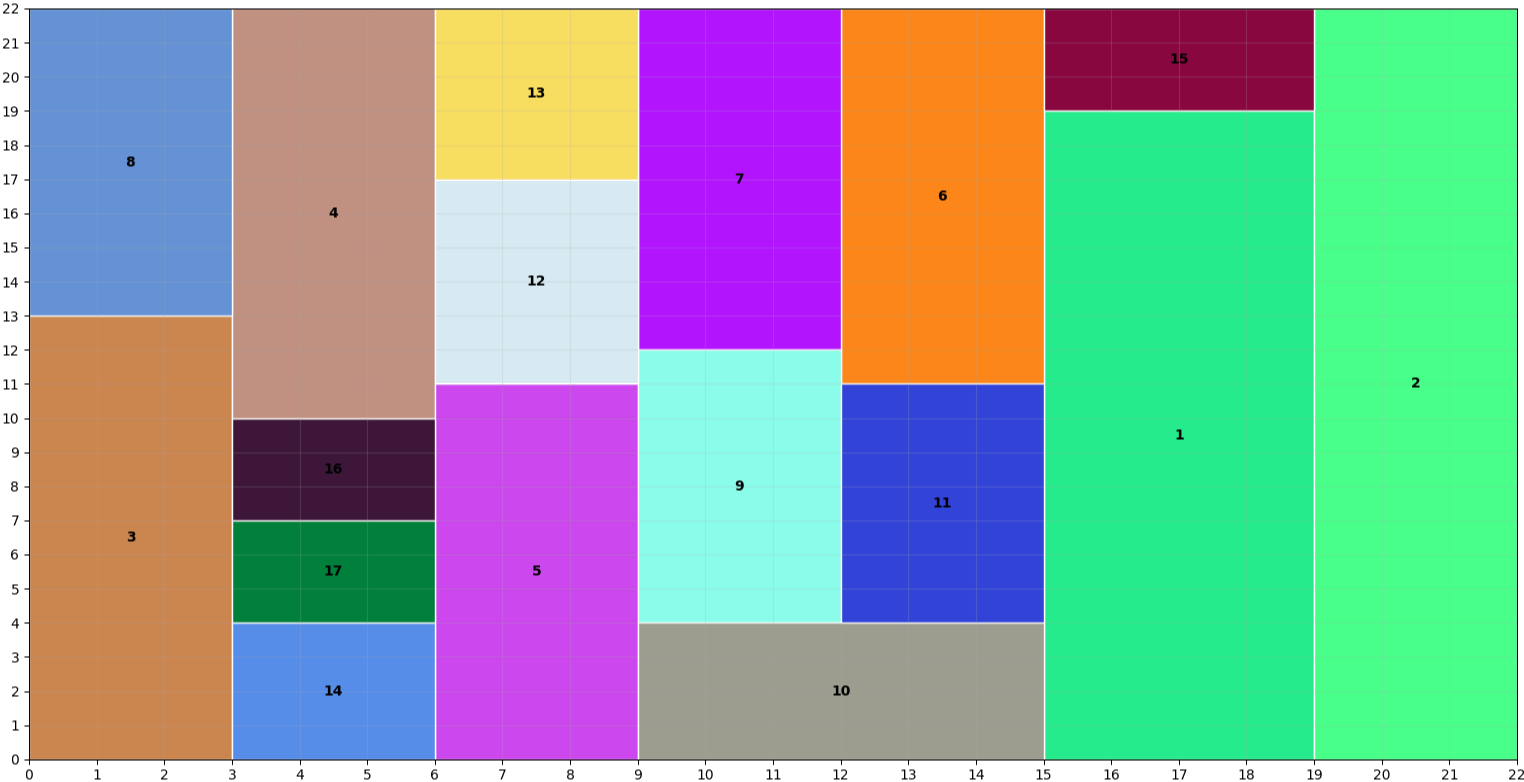
\includegraphics[width=\textwidth]{ins_15.png}
                \caption{}
                \label{fig:ins_15_mod}
            \end{subfigure}
            \hfill
            \begin{subfigure}[b]{0.45\textwidth}
                \centering
                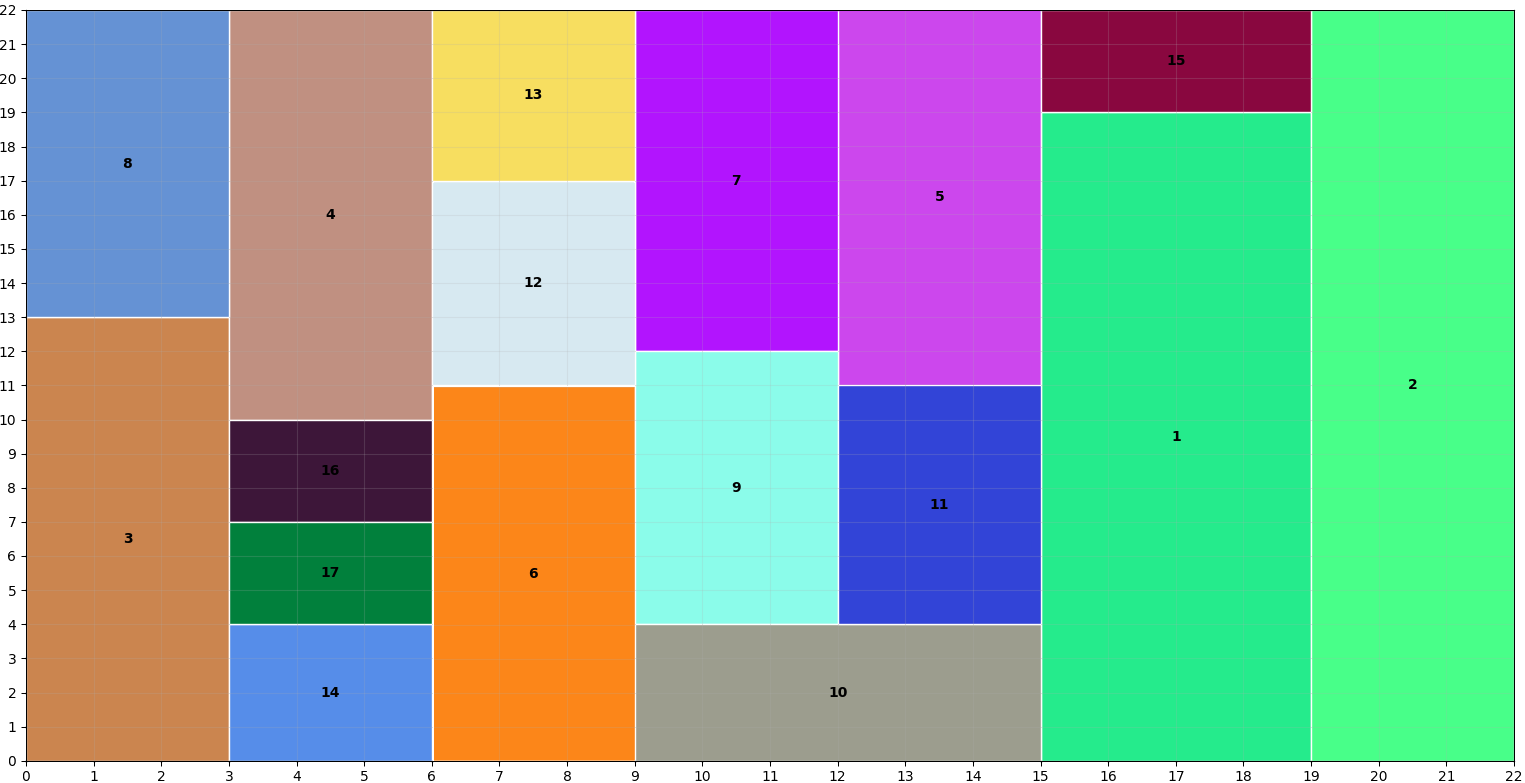
\includegraphics[width=\textwidth]{ins_15_swap.png}
                \caption{}
                \label{fig:ins_15_swap}
            \end{subfigure}
            \hfill
            \caption{
                Plotted solution of an instance created for explanatory puropose.
                From the solution on the left \ref{fig:ins_15_mod} we can create a different one
                with the same \textit{makespan} just swapping circuits with same dimensions. In
                the plot on the right \ref{fig:ins_15_swap} we swapped circuit 5 (at originial
                position of (6,0)) and circuit 6 (at originial position of (12,11)).
            }
            \label{fig:symmetry_swap}
        \end{figure}
       
        \begin{figure}[H]
            \centering
            \begin{subfigure}[b]{0.45\textwidth}
                \centering
                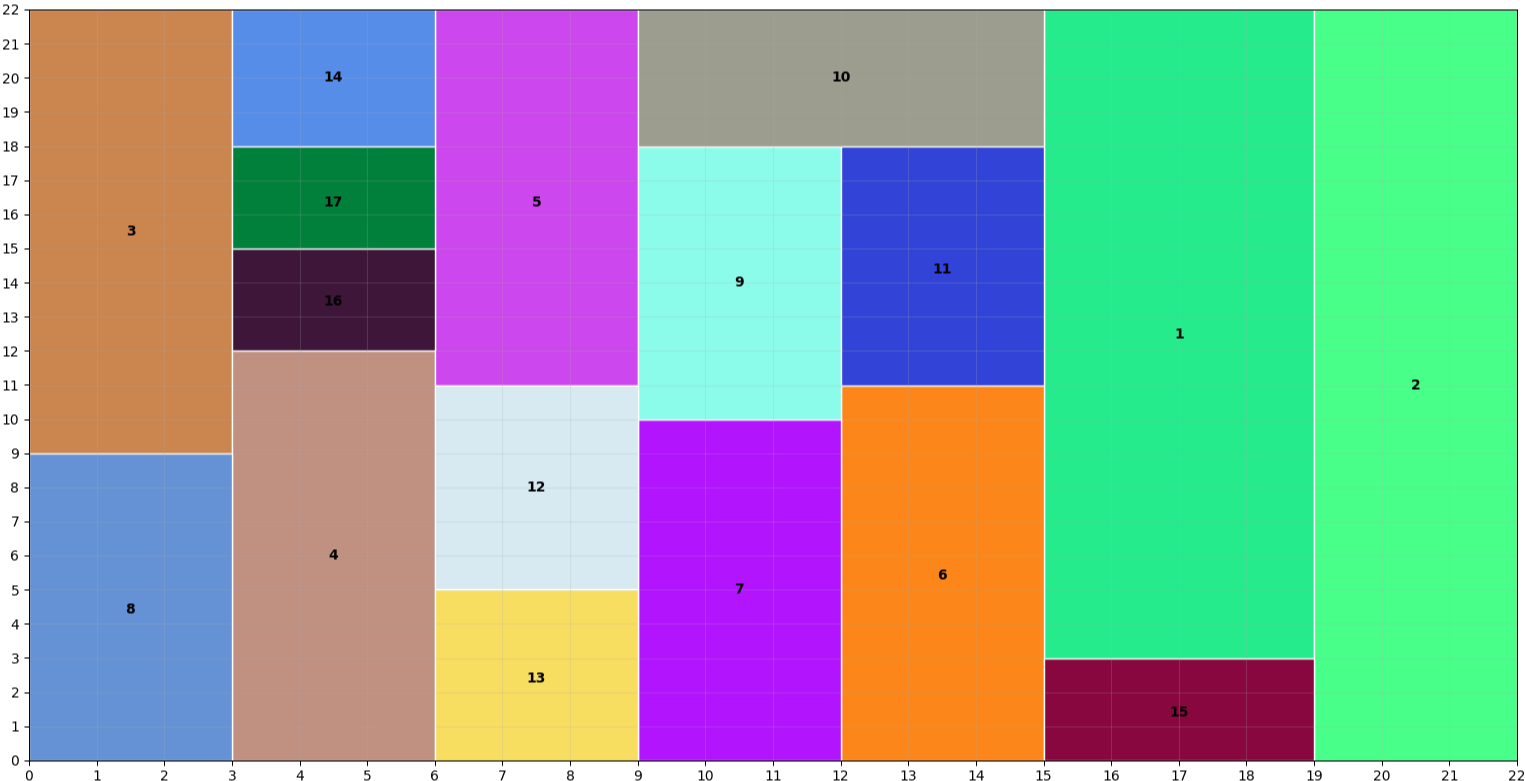
\includegraphics[width=\textwidth]{ins_15_specular_v.png}
                \caption{}
                \label{fig:ins_15_specular_v}
            \end{subfigure}
            \hfill
            \begin{subfigure}[b]{0.45\textwidth}
                \centering 
                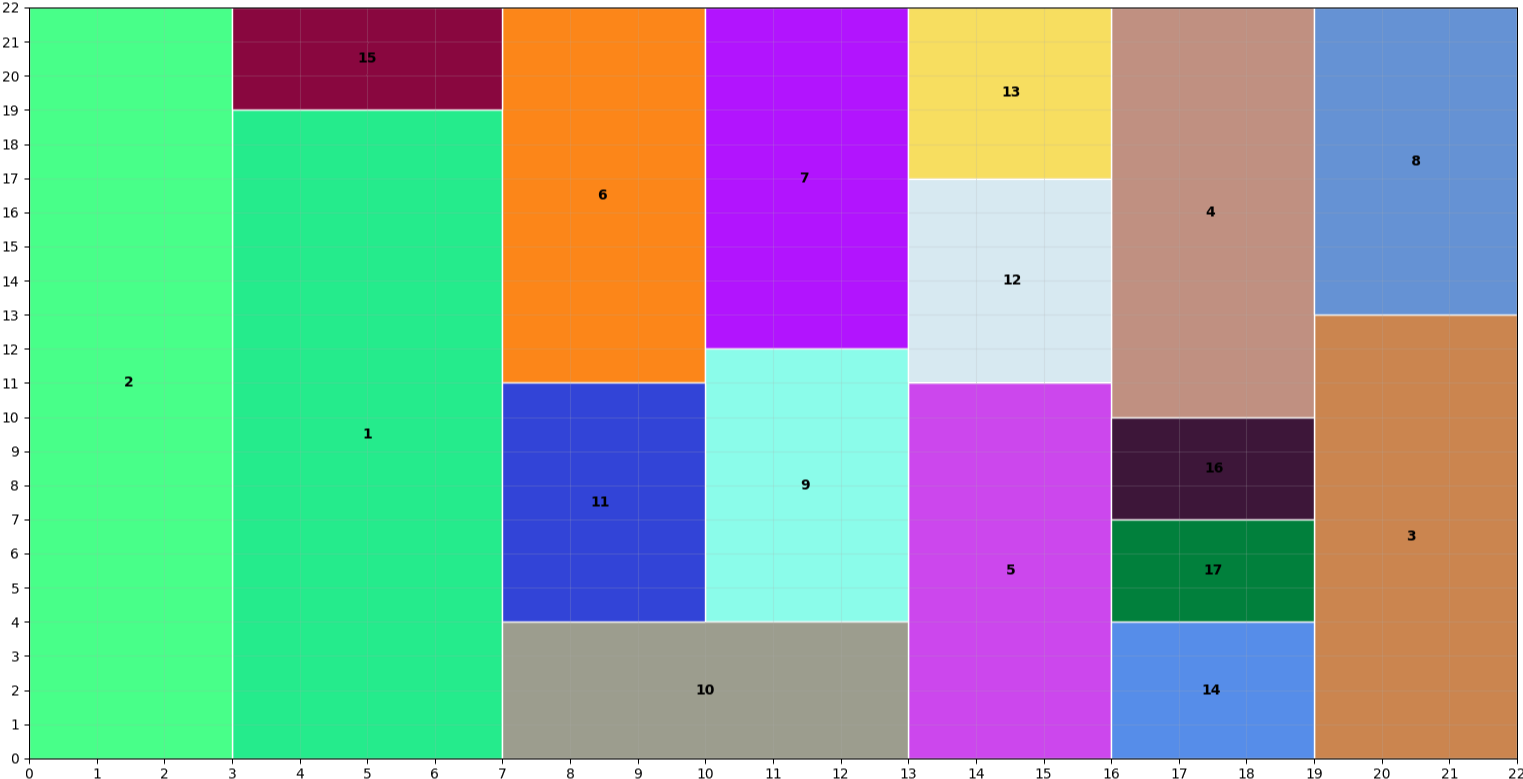
\includegraphics[width=\textwidth]{ins_15_specular_h.png}
                \caption{}
                \label{fig:ins_15_specular_h}
            \end{subfigure}
            \hfill
            \caption{
                Other possible solutions with same makespan as the one plotted in \ref{fig:ins_15_mod}.
                The left one \ref{fig:ins_15_specular_h} is the specular w.r.t. the vertical axis,
                while the left one \ref{fig:ins_15_specular_v} is the specular w.r.t. the horizontal axis
            }
            \label{fig:symmetry_specular}
        \end{figure}

        \begin{figure}[H]
            \centering
            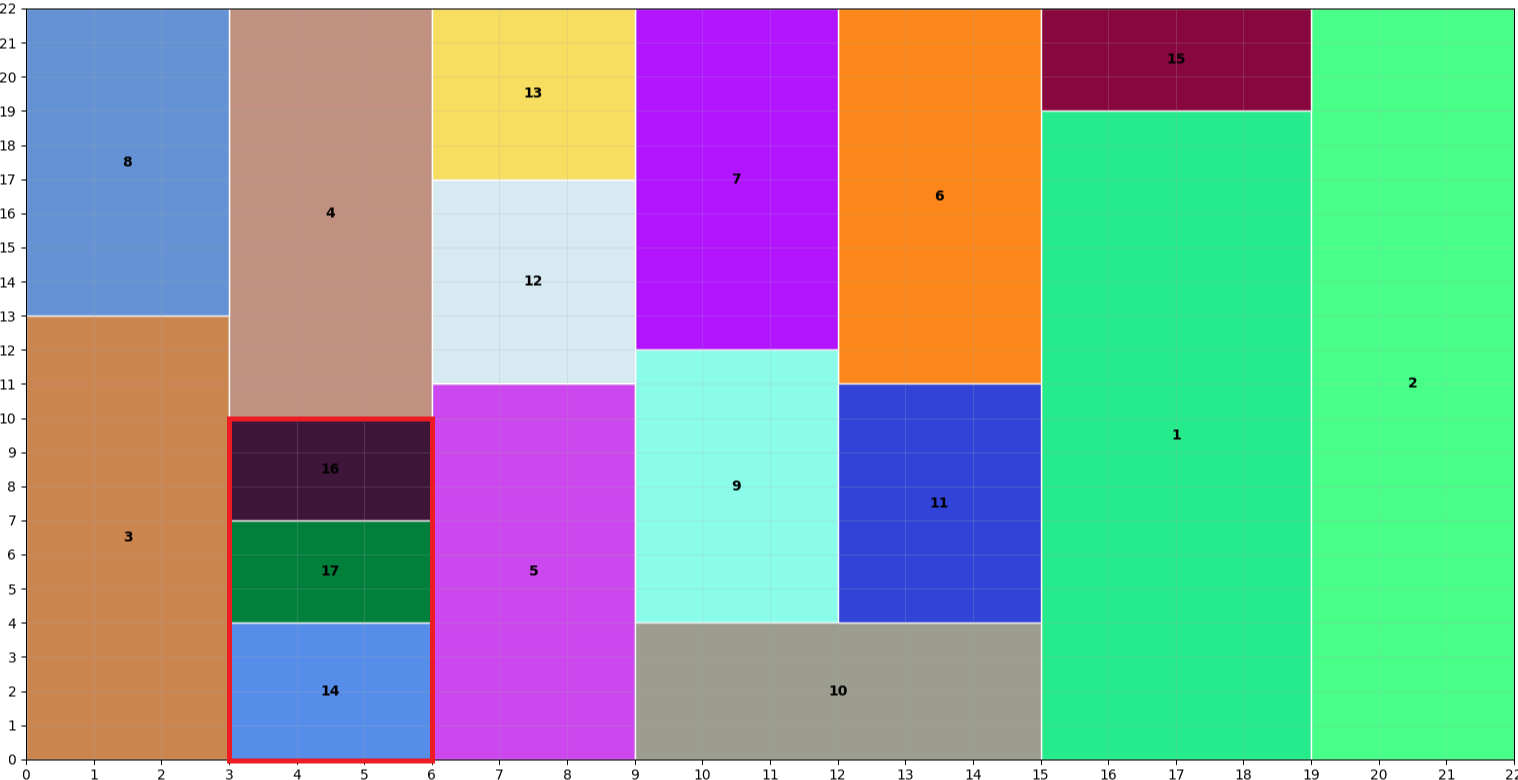
\includegraphics[width=0.5\textwidth]{ins_15_vc.png}
            \caption{
                At position $(3,0)$ an example of \textit{virtual} circuit highlighted in red,
                with $w = 3$ and $h = 10$, which includes inside the circuits 14, 16 and 17.
            }
            \label{fig:virtual circuit}
        \end{figure}

        \begin{figure}[H]
            \centering
            \begin{subfigure}[b]{0.3\textwidth}
                \centering 
                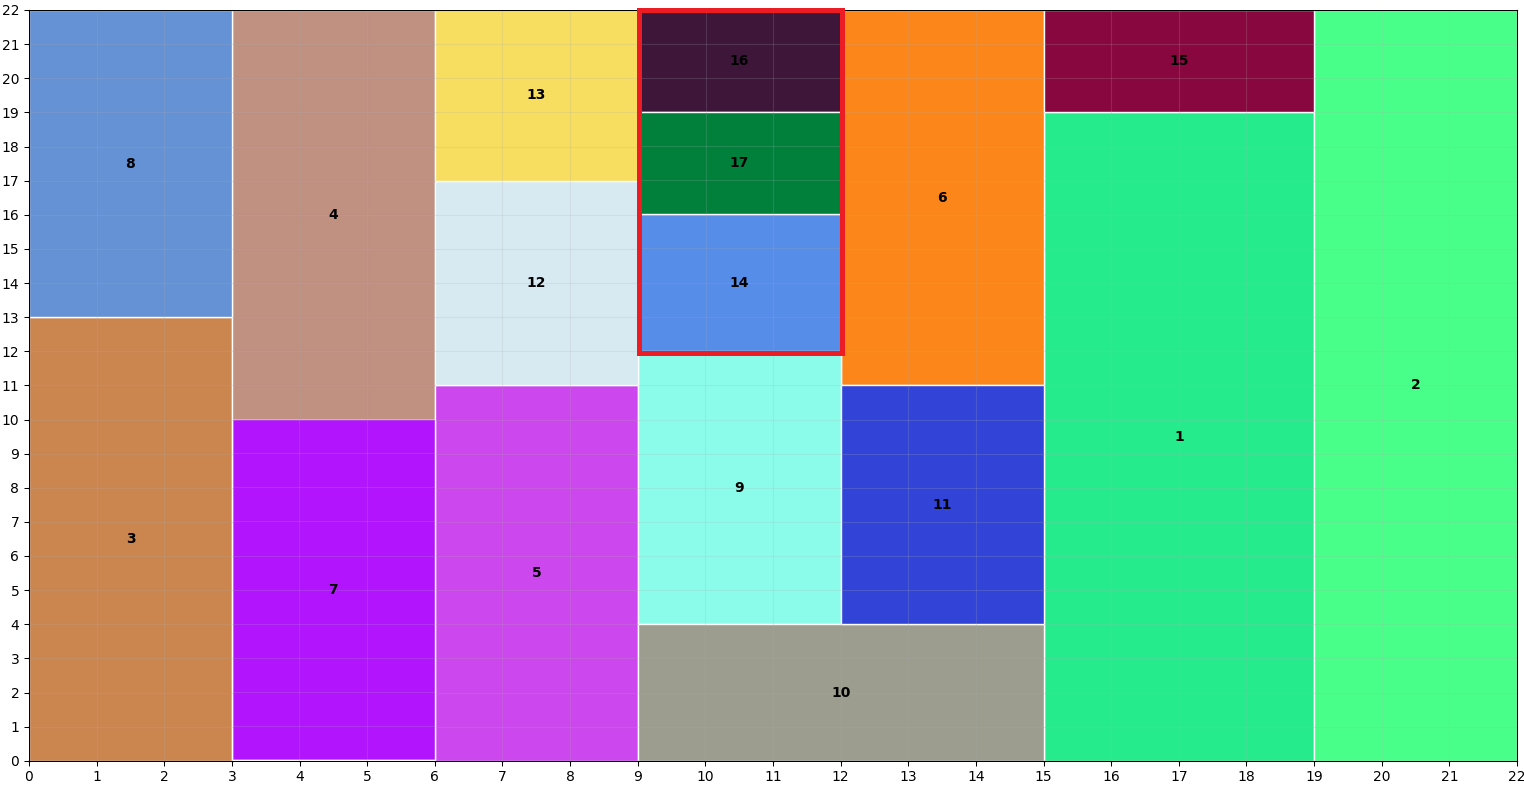
\includegraphics[width=\textwidth]{ins_15_vc_swap.png}
                \caption{}
                \label{fig:vc_swap}
            \end{subfigure}
            \hfill
            \begin{subfigure}[b]{0.3\textwidth}
                \centering
                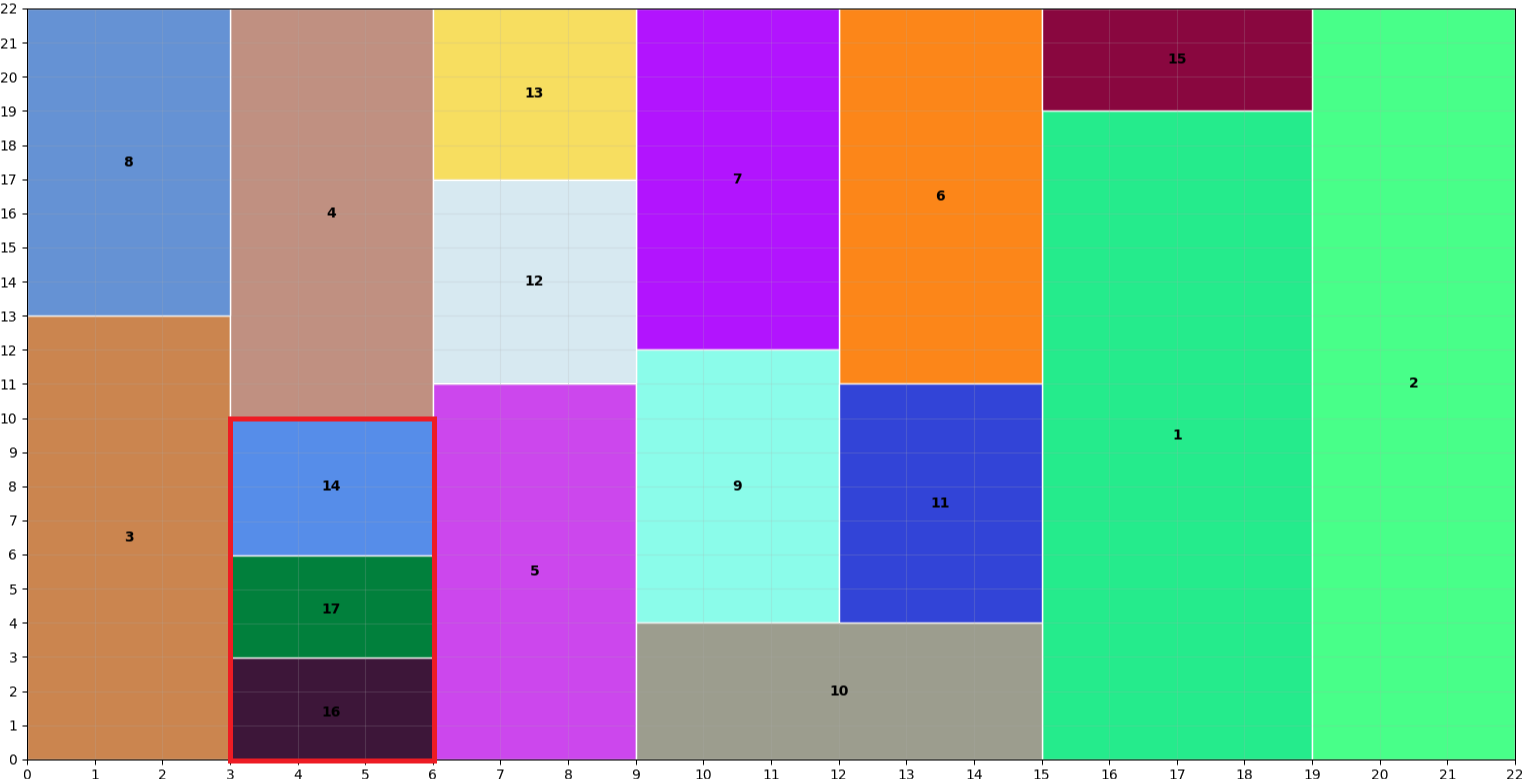
\includegraphics[width=\textwidth]{ins_15_vc_specular_in.png}
                \caption{}
                \label{fig:vc_specular_in}
            \end{subfigure}
            \hfill
            \begin{subfigure}[b]{0.3\textwidth}
                \centering
                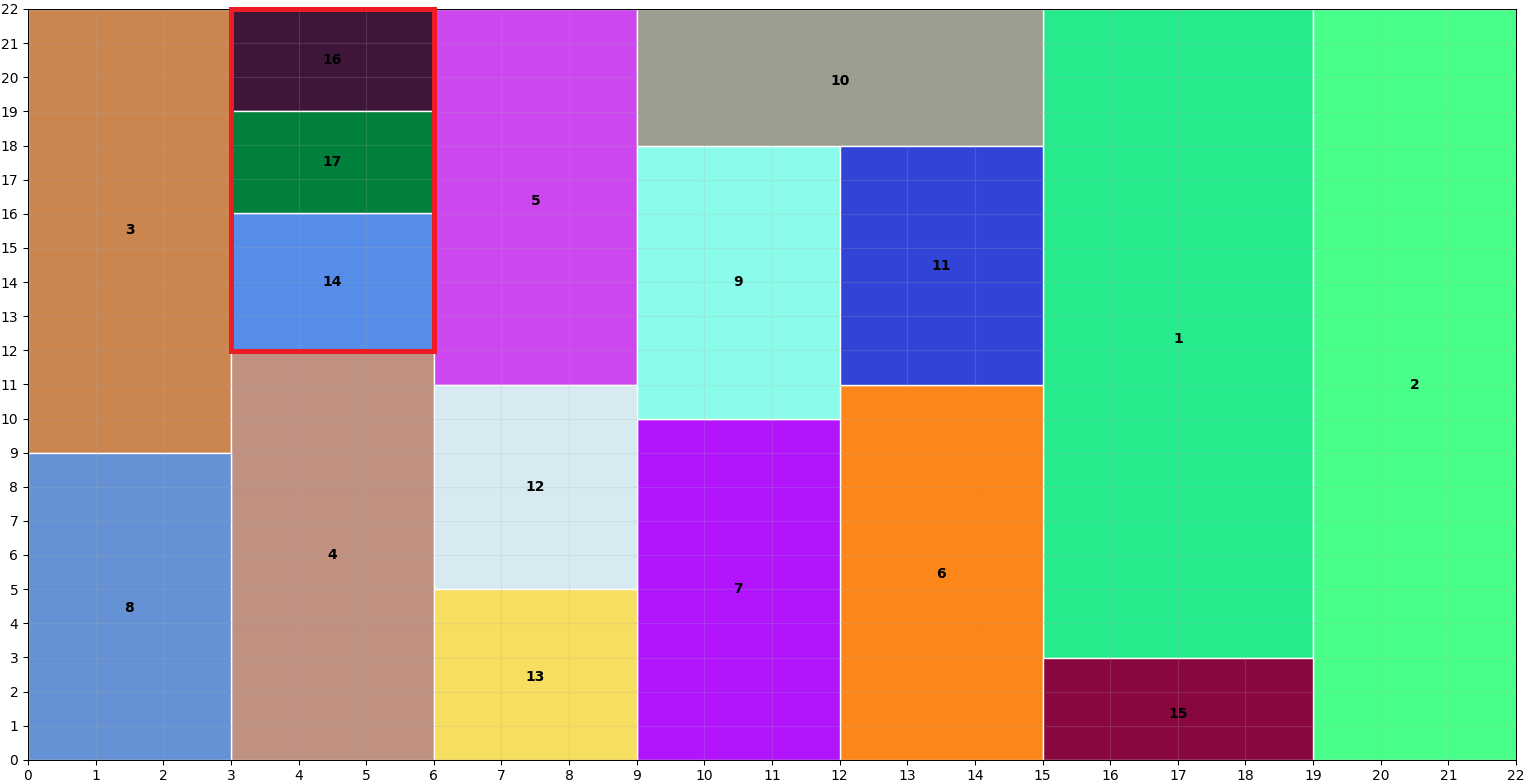
\includegraphics[width=\textwidth]{ins_15_vc_specular_out.png}
                \caption{}
                \label{fig:vc_specular_out}
            \end{subfigure}
            \caption{
                Other possible solutions with same makespan as the one plotted in \ref{fig:ins_15_mod},
                now including also \textit{virtual} circuits in the reasoning.
                In the left one \ref{fig:vc_swap}, the \textit{virtual} circuit introduced in \ref{fig:virtual circuit}
                at original position (3,0) is swapped with the regular circuit 7 at original position (9,11).
                In the middle one \ref{fig:vc_specular_in} the same \textit{virtual} circuit is substituted with 
                its specular w.r.t. the horizontal axis.
                The right one \ref{fig:vc_specular_out} is an example of combination of what mentioned before:
                starting from the solution \ref{fig:ins_15_specular_v}, the subset of circuits 14, 16, 17, belonging to 
                the highlighted \textit{virtual} circuit, is \textit{"mirrored"} again.
            }
            \label{fig:symmetry_vc}
        \end{figure}

        Catching all the symmetric solutions described before is quite demanding and we did not find an 
        efficient way of implementing symmetry breaking constraints, so we tried to keep them as simple 
        as possible.

        Let's define first some support variables:
        \begin{align*}
            x\_v\   &\ =\ [x_c\ |\ c \in C]                     \\
            y\_v\   &\ =\ [y_c\ |\ c \in C]                     \\
            x\_v'\  &\ =\ [width - (x_c + w_c)\ |\ c \in C]     \\
            y\_v'\  &\ =\ [makesapan - (y_c + h_c)\ |\ c \in C] \\ 
            \label{eq:specular_coord}
        \end{align*}
        where $x\_v$ and $y\_v$ are respectively the vector of all horizontal and vertical coordinates,
        while $x\_v'$ and $y\_v'$ are the horizontal and the vertical coordinates of the specular circuits.

        The symmetry breaking constraints proposed for CP, SAT and SMT are the lexicographic orderings
        between $y\_v$ and $y\_v'$ and between $x\_v$ and $x\_v'$; in this way we break the 
        symmetries shown respectively in Fig.\ref{fig:ins_15_specular_v} and Fig.\ref{fig:ins_15_specular_h}.

        Anyway, later we will specify better the adopted constraints and compare the performances of the 
        CP, SAT and SMT models with and without the symmetry breaking constraints.
